\chapter{Guía para el desarrollador: creación de juegos para BreakBrain}
\label{chap::guia}

\drop{E}{ste} apéndice pretende ser una guía completa para desarrolladores. A lo largo del mismo se detallará el funcionamiento interno del subsistema de juegos de BreakBrain y se explicará, de forma clara y utilizando ejemplos prácticos, el procedimiento de creación e integración de juegos de terceros en BreakBrain.

Tras la lectura de esta guía, el desarrollador estará en disposición de extender la funcionalidad de BreakBrain mediante sus propios juegos, ya sean monojugador o multijugador, posibilitando que cualquier usuario de la red social haga uso de ellos.

\section{Requisitos}

Antes de poder desarrollar un juego para BreakBrain existen algunos requisitos que el desarrollador debe satisfacer. Suponen la posesión de una serie de conocimientos, habilidades y herramientas necesarias para desarrollar juegos HTML5 2D compatibles con la plataforma.

\subsection{Conocimientos del desarrollador}

Para desarrollar juegos para BreakBrain es necesario:

\begin{itemize}
\item Conocimiento avanzado del lenguaje JavaScript.
\item Experiencia desarrollando con NodeJS.
\item Experiencia en desarrollo de gráficos 2D.
\item Conocimiento avanzado del canvas de \acs{HTML} y manejo fluido del \acs{DOM}.
\end{itemize}

Además, resulta recomendable contar con:

\begin{itemize}
\item Experiencia utilizando el framework de juegos 2D CreateJS.
\item Experiencia en el desarrollo de aplicaciones web de tiempo real.
\item Experiencia en el manejo de websockets.
\end{itemize}

\subsection{Herramientas de desarrollo}

En cuanto a las herramientas necesarias para desarrollar juegos para BreakBrain, encontramos las siguientes:

\begin{itemize}
\item Editor de texto plano: puede servir cualquier editor de texto, aunque es recomendable contar con algún editor avanzado que ofrezca resaltado de sintaxis y facilidades para la programación. Se recomienda GNU Emacs, pero puede utilizar otras soluciones, como VIM, Sublime Text, Gedit, etc.
\item Navegador web: necesario para depurar y probar los juegos en desarrollo. Resulta muy importante que el navegador que utilicemos disponga de buenas herramientas para facilitar la depuración, así como de un buen motor de JavaScript que permita sacarle todo el potencial gráfico a la máquina. Se recomienda utilizar Chromium/Chrome o Mozilla Firefox.
\item Terminal de línea de comandos para ejecutar NodeJS: este {\it runtime} es el utilizado para ejecutar la parte servidora de los juegos, por lo que resulta esencial disponer de él para asegurar el correcto funcionamiento del juego.
\end{itemize}

Aunque no es necesario, además se recomienda disponer de:

\begin{itemize}
\item Sistema Operativo de tipo UNIX: para el desarrollo y la ejecución de los juegos es altamente recomendable un entorno UNIX, como GNU/Linux, BSD o Mac OS X. 
\end{itemize}

\section{Tipos de juegos}

Cada juego de la plataforma pertenece y está diseñado para estimular a una única habilidad mental (ver tabla \ref{table:capacidades}). Por ello, antes de crear un juego el primer paso es decidir a qué habilidad mental estará dirigido. Independientemente de ello, el segundo paso será decidir el tipo de juego: en BreakBrain hay dos tipos de juegos, en función del número de jugadores que puedan participar en una misma partida: juegos monojugador y juegos multijugador.

\subsection{Juegos monojugador}

Se trata de juegos diseñados para ser utilizados por un único usuario, por lo que no supone ningún tipo de interacción social. En este tipo de juegos no se gana o se pierde, sino que el resultado es un valor cuantitativo que indica el grado de éxito de la partida, basado en la puntuación obtenida en cada actividad puntuable de la misma.

Para comprender mejor la relación entre los conceptos de juego, partida y actividad puntuable, ver sección \ref{sec::juegos-partidas-actividades}.

\subsection{Juegos multijugador}

En este caso se trata de juegos diseñados para ser utilizados por dos jugadores a la vez, suponiendo un enfrentamiento entre ellos. Sólo un jugador de los dos puede ganar cada ronda o partida. No obstante, el progreso del entrenamiento cerebral de ambos se verá afectado por el resultado que han obtenido en las actividades puntuables completadas durante la partida, independientemente de quién gane.

Para comprender mejor la relación entre los conceptos de juego, partida y actividad puntuable, ver sección \ref{sec::juegos-partidas-actividades}.

\section{El sistema de juegos de BreakBrain}

Llegados a este punto resulta conveniente comprender la composición del subsistema de juegos de la plataforma, así como de cada juego de la misma.

\subsection{Componentes del sistema de juegos}

El sistema de juegos de BreakBrain se compone de tres elementos, o conjuntos de elementos, bien diferenciadas:

\begin{itemize}
\item Cargador de juegos
\item Partes servidoras de los juegos
\item Partes cliente de los juegos
\end{itemize}

El cargador de juegos es la piedra angular del subsistema, ya que se encarga de chequear los juegos disponibles y ponerlos a disposición del usuario. Una vez instalado correctamente un nuevo juego en una instancia de BreakBrain, el cargador se encargará de analizar sus componentes, arrancar la parte servidora del mismo y poner a disposición de la web la parte cliente, para que cualquier usuario pueda usarlo. Todo ello tiene lugar de forma automática.

Las partes servidoras de los juegos se encuentran en el lado del servidor. El cargador de juegos arranca dichas partes servidoras en el proceso de inicio del servidor, para que los juegos estén disponibles y las partes cliente puedan comunicarse con las partes servidoras.

Las partes cliente de los juegos se cargan de forma dinámica al abrir la web de BreakBrain. Son más flexibles, en el sentido en el que no requieren de un reinicio del servidor para funcionar o manifestar cambios.

\subsection{Componentes de un juego}

Los juegos de BreakBrain se componen de 2 partes principales: un pequeño servidor (un único script JS) y un cliente (un directorio con un script JS y recursos).

\subsubsection{Parte servidora}

La parte servidora de los juegos es ejecutada en un servidor NodeJS. Se trata de la espina dorsal sobre la que el juego se construye. En el caso de juegos monojugador, este componente es muy sencillo, y se limita a almacenar el resultado de las partidas mediante llamadas al núcleo del servidor de BreakBrain. En el caso de partidas multijugador, el papel es aún más importante, encargándose de la lógica del juego, la comunicación con la parte cliente de los jugadores y manteniendo la sincronización constante.

Tal y como BreakBrain está concevido, las tareas mencionadas resultan realmente sencillas: la conexión con los clientes se gestiona de forma automática, sin que el desarrollador tenga que preocuparse por ello. La comunicación resulta trivial. La lógica principal del juego dependerá de qué clase de juego se implemente.

En la sección \ref{sec::creacion-juego} se detalla el proceso de creación de un juego desde cero, detallando el comportamiento de la parte servidora de un juego.

\subsubsection{Parte cliente}

La parte cliente de los juegos es ejecutada por el navegador web. La experiencia de usuario puede variar, por lo tanto, dependiendo del navegador web del usuario de BreakBrain. El papel de la parte cliente de los juegos es gestionar la representación gráfica del estado y evolución de los mismos. En juegos monojugador, además, la lógica del juego puede estar implementada en este componente (dado que no se comparte con otros usuarios en tiempo de ejecución).

En la sección \ref{sec::creacion-juego} se detalla el proceso de creación de un juego desde cero, detallando el comportamiento de la parte cliente de un juego.

\subsubsection{Recursos}

Los recursos multimedia requeridos por los juegos (sprites, archivos de audio, etc.) se localizan en la parte cliente ---dado que es la que los utiliza---. Como mínimo un fondo o background y un icono son obligatorios por juego.

\section{Creación de un juego desde cero}
\label{sec::creacion-juego}

En esta sección se realizará un recorrido práctico por el proceso de creación de un juego. Para ello se creará un juego completo desde cero.

\subsection{Eligiendo una categoría}

El primer paso a la hora de crear un juego para BreakBrain es elegir la categoría a la que se quiere que pertenezca, es decir, la capacidad y habilidad mental que se quiere entrenar. En BreakBrain cada juego se orienta a la estimulación de una única habilidad mental (perteneciente a una única categoría).

A continuación se listan las capacidades en las que el entrenamiento cerebral se divide, así como las habilidades mentales que componen cada una de ellas.

\begin{itemize}
\item Memoria
  \begin{itemize}
  \item Memoria de trabajo
  \item Memoria espacial
  \item Memoria nombre-cara
  \end{itemize}

\item Resolución de problemas
  \begin{itemize}
  \item Aritmética
  \item Razonamiento lógico
  \item Razonamiento cuantitativo
  \end{itemize}

\item Atención
  \begin{itemize}
  \item Concentración
  \item Campo visual
  \end{itemize}

\item Velocidad
  \begin{itemize}
  \item Procesamiento de información
  \item Orientación espacial
  \end{itemize}

\item Flexibilidad
  \begin{itemize}
  \item Control de impulsos
  \item Planificación
  \item Conmutación de tareas
  \item Fluidez verbal
  \end{itemize}
\end{itemize}

En la tabla \ref{table:capacidades} se ofrece una sencilla descripción de cada habilidad mental, junto a una explicación del funcionamiento de un juego basado en ella.

En esta guía se seguirán los pasos necesarios para crear un juego orientado a mejorar la habilidad {\bf Memoria nombre-cara} de la capacidad {\bf Memoria}. El juego se llamará, por ejemplo, ``Careto''.

\begin{figure}[H]
  \begin{center}
    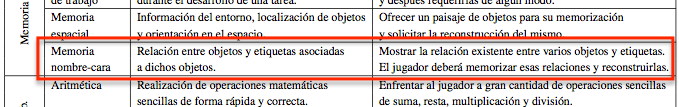
\includegraphics[width=1\textwidth]{images/captura-nombre-cara.png}
  \end{center}
\end{figure}

El juego ofrecerá al jugador una serie de objetos con una etiqueta asociada durante unos segundos. Después se mostrarán los objetos sin etiquetas, y el jugador deberá especificar la etiqueta de cada uno de ellos. Las etiquetas que serán asociadas a cada objeto no tendrán relación semántica alguna con él, para evitar que el conocimiento previo a la partida pueda influir en el resultado de la misma.

\subsection{Eligiendo el tipo de juego}

Los juegos para BreakBrain pueden ser monojugador o multijugador. Ambos tipos de juegos servirán del mismo modo al entrenamiento cerebral, pero en el caso de los juegos multijugador entrará en juego, además, el aspecto social y motivante del enfrentamiento a otro usuario.

En este caso se optará por la creación de un juego multijugador. Ambos jugadores serán enfrentados a la misma escena, para asegurar la igualdad de condiciones, y cuando uno la consiga resolver ambos pasarán a la siguiente. Nótese que este tipo de decisiones dependen del desarrollador, y en este mismo caso podría decidirse enfrentar a los dos jugadores a diferentes escenas, independizando el progreso de cada uno en la partida.

\subsection{Creando la estructura básica del juego}

¡Manos a la obra! Es hora de empezar a crear el juego. En este paso es totalmente recomendable tener instalado BreakBrain en local, para poder depurar el juego durante el desarrollo, sin tener que esperar a terminarlo. Así pues, suponiendo que tenemos una copia funcionando en el directorio {\tt \$BREAKBRAIN}, tendremos que seguir los siguientes pasos para crear la estructura del juego:

\begin{enumerate}
\item Crear el script de servidor. Por seguir la nomenclatura de la plataforma habrá que llamarlo de la forma ``{\tt <nombreEnCamelCase>-server.js}''. Dicho script debe situarse en el directorio de partes servidoras de juegos ({\tt \$BREAKBRAIN/server/games}). En nuestro caso:
  \begin{center}
    {\tt \$BREAKBRAIN/server/games/careto-server.js}
  \end{center}

\item Ahora se debe crear el directorio de la parte cliente del juego. Se sigue la misma nomenclatura: ``{\tt <nombreEnCamelCase>-client}''. La ubicación adecuada es el directorio donde se encuentran las partes clientes de los juegos: {\tt \$BREAKBRAIN/public/games}. En nuestro caso, el directorio a crear es el siguiente:
  \begin{center}
    {\tt \$BREAKBRAIN/public/games/careto-client}
  \end{center}

\item Crear el script cliente del juego (llamado {\tt main.js}) en su directorio cliente. En nuestro caso, el script se sitúa en:
  \begin{center}
    {\tt \$BREAKBRAIN/public/games/careto-client/main.js}
  \end{center}

\item Especificar un icono y una imagen de fondo para el juego. Estas dos imágenes deben ubicarse en el directorio de la parte cliente del juego, y se llamarán {\tt logo.png} y {\tt background.png}, respectivamente. El logo debe tener un tamaño de 125x125 pixels, y el fondo de 600x480 pixels. En nuestro caso, ambos archivos son los siguientes:
  \begin{center}

    {\tt \$BREAKBRAIN/public/games/careto-client/logo.png}\\

    \begin{figure}[H]
      \begin{center}
        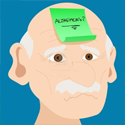
\includegraphics[scale=0.7]{images/careto-logo.png}
        \caption{Logo del juego ``Careto''}
      \end{center}
    \end{figure}

    {\tt \$BREAKBRAIN/public/games/careto-client/background.png}

    \begin{figure}[H]
      \begin{center}
        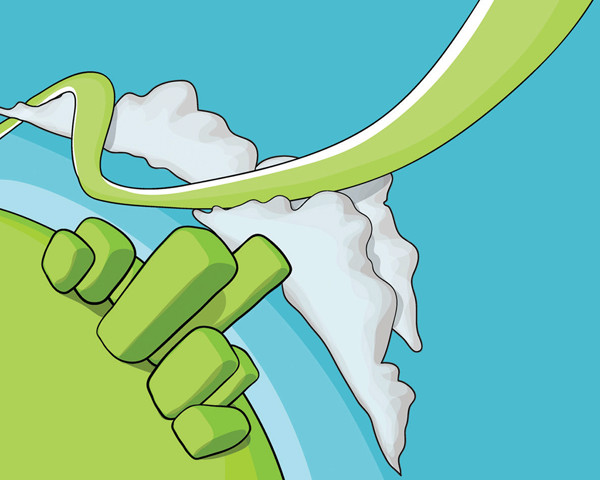
\includegraphics[scale=0.5]{images/careto-background.png}
        \caption{Fondo del juego ``Careto''}
      \end{center}
    \end{figure}
  \end{center}

\end{enumerate}

\subsection{Preparando los recursos}

Cualquier recurso multimedia empleado por el juego deberá situarse en el directorio de su parte cliente. En nuestro caso:
\begin{center}
  {\tt \$BREAKBRAIN/public/games/careto-client}
\end{center}

Para ``Careto'' utilizaremos una serie de imágenes (a las que asociaremos una etiqueta durante la ejecución). La etiqueta será textual, por lo que no necesita ningún recurso externo. Las imágenes, por otro lado, deberán ser incluidas como recurso externo. En este caso se emplearán las letras del alfabeto Braille como imágenes a las que asociar las etiquetas (ver figura \ref{fig::braille}).

\begin{figure}[h]
  \begin{center}
    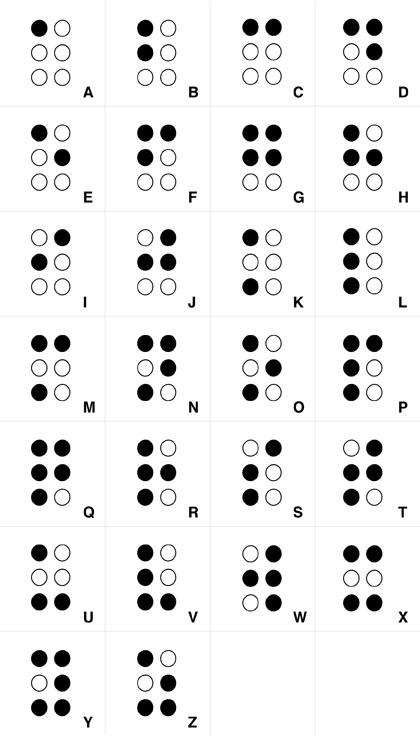
\includegraphics[width=0.5\textwidth]{images/braille.jpg}
    \caption{Imágenes de juego para ``Careto''}
    \label{fig::braille}
  \end{center}
\end{figure}

Llegados a este punto, la estructura y recursos de ``Careto'' están perfectamente definidas y ubicadas en su localización correcta:

\begin{figure}[H]
  \begin{center}
    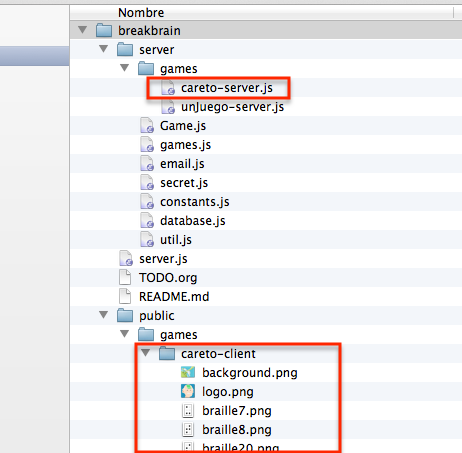
\includegraphics[width=0.8\textwidth]{images/careto-jerarquia.png}
    \caption{Jerarquía de directorios para ``Careto''}
  \end{center}
\end{figure}

\subsection{Desarrollando la parte servidora}

El esquema de la parte servidora de un juego de BreakBrain es realmente sencillo, y es el mostrado en el listado \ref{code::game-server-scheme}. Basta con importar la clase {\tt Game} y exportar una función que devuelva una instancia de dicha clase. La función puede recibir 2 argumentos que BreakBrain pasa automáticamente:

\begin{itemize}
\item Una función de test que se puede utilizar para realizar tests unitarios del juego.
\item La URL esperada de la parte cliente (esta debe pasarse a su vez a la instancia de {\tt Game}).
\end{itemize}

La recepción de estos dos argumentos es opcional, pero recomendable. La función de test es realmente útil para ejecutar tests unitarios. Por otro lado, la ruta de la parte cliente puede establecerse a mano, pero no hay razón para ello si se siguen las directivas establecidas de ubicación y nomenclatura.

\newpage
\begin{lstlisting}[frame=single, language=JavaScript, caption={Esquema de la parte servidora de un juego para BreakBrain}, label=code::game-server-scheme]
var Game = require('../Game.js');

module.exports = function (test, clientURL) {

    var g = new Game(
        'Careto',              // Nombre del juego
        'Memoria',             // Capacidad a estimular
        'Memoria nombre-cara', // Habilidad mental
        clientURL              // URL de la parte (auto)
    );

    // Puede utilizar el framework de pruebas incluido
    // en BreakBrain para realizar test unitarios:
    // 
    // test('Nombre del test', <condicion>, 'mensaje de fallo');

    setInterval(function(){

        // Aqui la logica periodica:
        //   - Actualizaciones del estado que dependan del tiempo
        //   - Comprobacion de si el juego se ha terminado

    }, 100);

    g.on = function (msg) {

        // Actualizar el estado del juego en funcion del mensaje
        // que llegue.
        //
        // El formato del mensaje se define en el cliente, pero
        // todos los mensajes incluyen un campo fijo: "from"
        // (el ID de usuario que envia el mensaje)

    };

    return g;
};
\end{lstlisting}

\subsection{Desarrollando la parte cliente}


\section{Publicación del juego en BreakBrain}









ljksdf
fs
df




aquí va un código

\begin{listing}[language=JavaScript, caption={Hola mundo en C}, label=code:hello]
var a = function(arg){
  console.log('hola' + arg); // Esto es un comentario
};
\end{listing}

